% !TEX root = ../lab4.tex
\section{Техническое задание}

Необходимо извлечь два последовательных кадра из видео и вычислить для них вектора смещений, используя метрику SAD или SSD. По найденным векторам смещения восстановить предыдущий кадр. Визуализировать результат. Исследовать влияние параметров блока и окна поиска на результат восстановления. 

\section{Ход работы}

\subsection{Описание алгоритма}

\begin{enumerate}
	\item Делим текущий кадр на равные блоки (NxN);
	\item Производим обход всех блоков текущего изображения, где для каждого блока производится обход некоторой окрестности блока в предыдущем кадре в поиске максимального соответствия (с помощью метрик SAD, SSD);
	\item  Таким образом, после завершения поиска мы получаем набор векторов, указывающих "`движение"' блоков между кадрами. С их помощью восстанавливаем предыдущий кадр.
\end{enumerate}

\begin{equation}
	SAD(d_1,d_2) = \sum_{i=0}^{n1}\sum_{j=0}^{n2}(d_1[i,j] - d_2[i,j])
\end{equation}

\begin{equation}
	SSD(d_1,d_2) = \sum_{i=0}^{n1}\sum_{j=0}^{n2}(d_1[i,j] - d_2[i,j])^2
\end{equation}

\subsection{Взятие последовательных кадров}

Напишем скрипт (листинг \vref{lst:getframes}) для взятия последовательных кадров из видео. В результате, в каталоге "`frames"' появилось определенное количество последовательных кадров, сохраненных в формате png. Для исследования выберем следующие:

\begin{figure}[H]
	\centering
	
\includegraphics[width=\textwidth]{frame639}
	\caption{Кадр T-1}
	\label{pic:frame639}
\end{figure}

\begin{figure}[H]
	\centering
	
\includegraphics[width=\textwidth]{frame640}
	\caption{Кадр T}
	\label{pic:frame640}
\end{figure}

\subsection{Вычисление векторов смещения и восстановления кадра}

Реализация алгоритма представлена в \vref{app:python}. Для исследования влияния параметров блока и окна поиска проведем следующие эксперименты (для всех случаев шаг поиска равен размеру блока):

Оценка влияния окна поиска:

Размер блока 16 на 16. Окно поиска 32 (64 на 64) 

\begin{figure}[H]
	\centering
	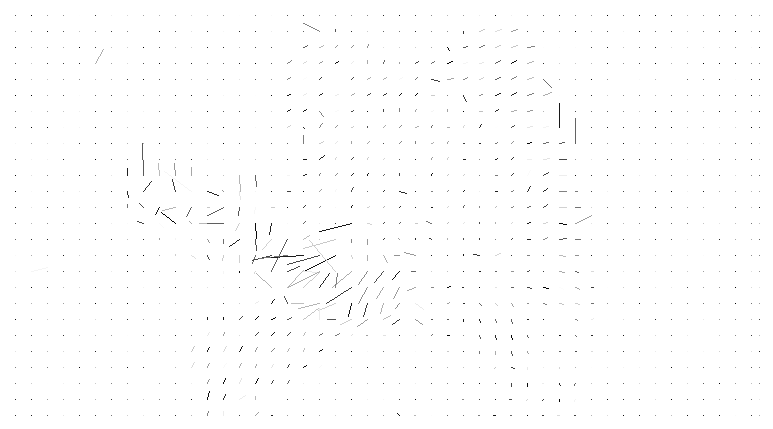
\includegraphics[width=\textwidth]{1}
	\caption{Векторы смещения (16x16, 64x64)}
	\label{pic:1}
\end{figure}

\begin{figure}[H]
	\centering
	\includegraphics[width=\textwidth]{2}
	\caption{Восстановленное изображение (16x16, 64x64)}
	\label{pic:2}
\end{figure}

Размер блока 16 на 16. Окно поиска 40 (80 на 80) 

\begin{figure}[H]
	\centering
	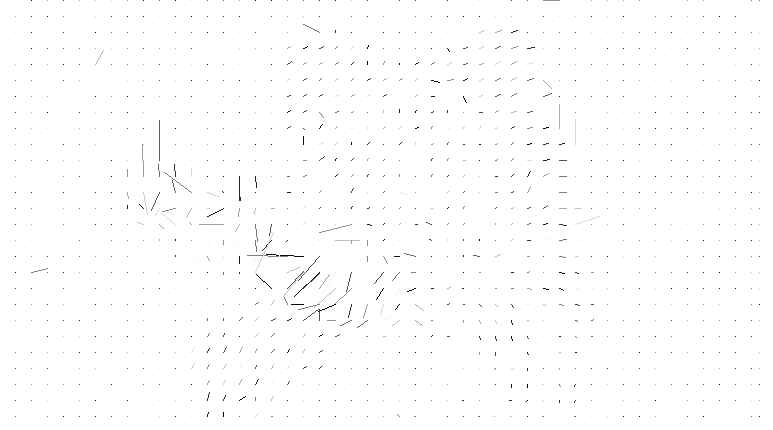
\includegraphics[width=\textwidth]{3}
	\caption{Векторы смещения (16x16, 80x80)}
	\label{pic:3}
\end{figure}

\begin{figure}[H]
	\centering
	\includegraphics[width=\textwidth]{4}
	\caption{Восстановленное изображение (16x16, 80x80)}
	\label{pic:4}
\end{figure}

Оценка влияния размера блока: 

Размер блока 8 на 8. Окно поиска 40 (80 на 80)

\begin{figure}[H]
	\centering
	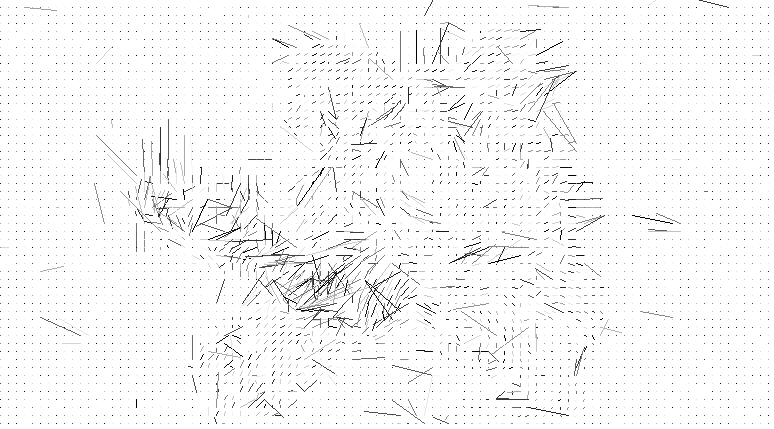
\includegraphics[width=\textwidth]{5}
	\caption{Векторы смещения (8x8, 80x80)}
	\label{pic:5}
\end{figure}

\begin{figure}[H]
	\centering
	\includegraphics[width=\textwidth]{6}
	\caption{Восстановленное изображение (8x8, 80x80)}
	\label{pic:6}
\end{figure}

Размер блока 5 на 5. Окно поиска 40 (80 на 80)

\begin{figure}[H]
	\centering
	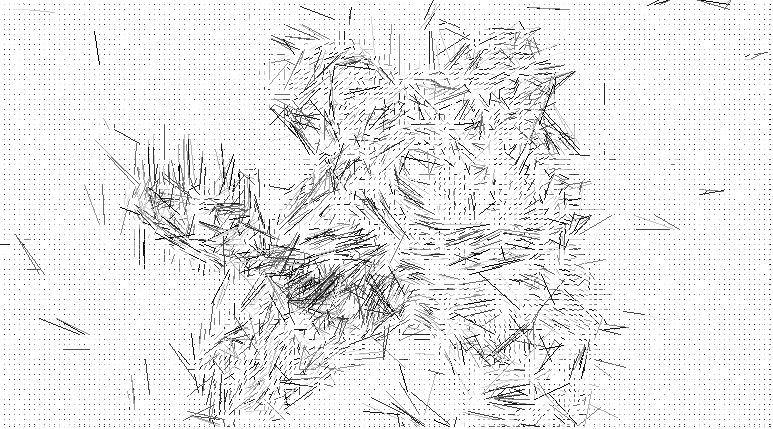
\includegraphics[width=\textwidth]{7}
	\caption{Векторы смещения (5x5, 80x80)}
	\label{pic:7}
\end{figure}

\begin{figure}[H]
	\centering
	\includegraphics[width=\textwidth]{8}
	\caption{Восстановленное изображение (5x5, 80x80)}
	\label{pic:8}
\end{figure}

Также попробуем провести поиск векторов смещения для кадра, сдвинутого на несколько пикселей вправо:

\begin{figure}[H]
	\centering
	\includegraphics[width=\textwidth]{9}
	\caption{Сдвинутое изображение}
	\label{pic:9}
\end{figure}

\begin{figure}[H]
	\centering
	
\includegraphics[width=\textwidth]{10}
	\caption{Векторы смещения (16x16, 64x64)}
	\label{pic:10}
\end{figure}

Как можно заметить, сдвиг большинства блоков был обнаружен корректно, некорректные векторы скорее всего вызваны идентичностью этих блоков, из-за чего произошло ложное срабатывание.

\section{Выводы}

Существуют разные методы компенсации движения в видео. Все они могут быть адаптированы под решение различного рода задач, например, для сжатия данных. Одним из наиболее популярных является блочный метод. Он позволяет по найденным векторам смещения восстанавливать изображение.

В ходе выполнения данной работы был проведен ряд экспериментов, из которых установлено, что такие параметры как "`размер блока"' и "`размер окна поиска"' оказывают наибольшее влияние на качество восстановления. Для тестовых фреймов было установлено, что при размере блока 5x5 и окна поиска 40x40 восстановление проходит почти без потери качества. Следует отметить, что параметр "`шаг поиска"' также влияет на качество изображения, однако для того чтобы его использование было целесообразно, необходимо реализовать качественный алгоритм для "`сложения"' пикселей (в данной работе при реализации используется среднее арифметическое). 

Как можно заметить, чем меньше размер блока, тем меньше фрагментация восстановленного изображения. Увеличение окна поиска вместе с уменьшением шага поиска обеспечивают большее количество потенциальных кандидатов на искомый блок, что увеличивает вероятность и точность его нахождения. Взамен все эти улучшения качества поиска увеличивают время его выполнения. 